%! TEX root = ../main.tex
% ============================================================
% IMMUTABLE — generated automatically, do not edit this block
%   script          : plotter.py::plot_fft_peak_bias_cancellation
%   plot_type       : fft_peak_bias_cancellation
%   chapter         : 04
%   panel           : None
%   wind            : None
%   amplitude       : None
%   frequency       : None
%   probes          : None
%   draft           : True
%   data            : analysis_scratch/fft_peak_bias_outin_impact.csv
%   n_runs          : 367
%
% SUBFIGURES AVAILABLE:
%   FIGURES/ch04_fft_peak_bias_cancellation.pdf
% ============================================================
\begin{figure}[htbp]
  \centering
  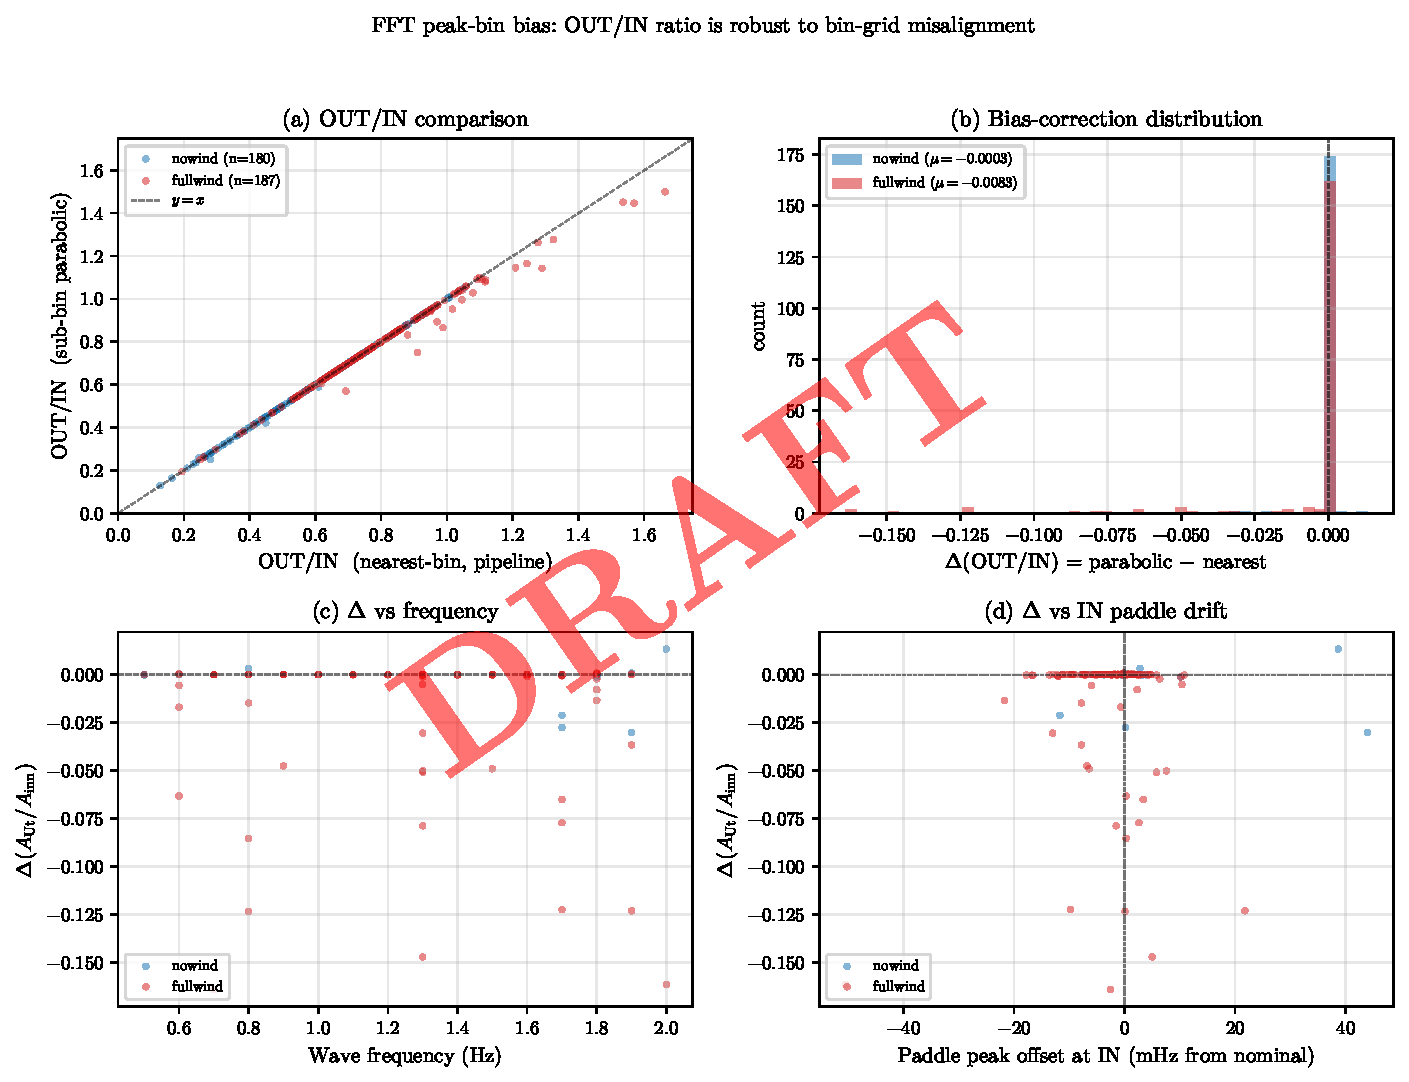
\includegraphics[width=0.9\linewidth]{FIGURES/ch04_fft_peak_bias_cancellation.pdf}
  \caption[Cancellation of the FFT peak-bin bias in the OUT/IN ratio (367 runs; nowind 180, fullwind 187)]{
    Cancellation of the FFT peak-bin bias in the OUT/IN ratio (367 runs; nowind 180, fullwind 187). Nearest-bin amplitude is systematically biased by paddle-drift vs FFT bin-grid alignment (sinc-attenuation up to ~40\,\% for individual amplitudes). Panel (a): OUT/IN computed with the pipeline's nearest-bin rule is near-identical to sub-bin parabolic-interpolated amplitude (y = x shown dashed). Panel (b): distribution of $\Delta(\mathrm{OUT/IN}) = \mathrm{parabolic} - \mathrm{nearest}$ is sharply peaked near zero. Panel (c): residual $\Delta$ has no strong frequency structure. Panel (d): $\Delta$ grows with the IN-probe paddle peak offset from nominal (the expected driver of sinc attenuation) but stays small because the OUT probe sees the same offset. Mean $|\Delta|/(\mathrm{OUT/IN}) = 0.46\,\%$; 95\,\% of runs have $|\Delta| < 0.02$; worst-case $|\Delta| = 0.164$. Fullwind introduces a small negative tail (mean $\Delta = -0.0083$ vs nowind -0.0003) from wind-induced spectral broadening at the IN probe. Conclusion: OUT/IN ratios are robust to the peak-bin bias; individual absolute amplitudes are not.
  }
  \label{fig:ch04_fft_peak_bias_cancellation}
\end{figure}
